% utf-8 ru, unix eolns
\documentclass[12pt,a4paper,oneside]{extarticle}
    \righthyphenmin=2 %минимально переносится 2 символа %%%
    \sloppy

%\title{Курсач: <<Молекулярное моделирование>>}

% Рукопись оформлена в соответствии с правилами оформления 
% электронной версии авторского оригинала, 
% принятыми в Издательстве МГТУ им. Н.Э. Баумана.

\usepackage{geometry} % А4, примерно 28-31 строк(а) на странице 
    \geometry{paper=a4paper}
    \geometry{includehead=false} % Нет верх. колонтитула
    \geometry{includefoot=true}  % Есть номер страницы
    \geometry{bindingoffset=0mm} % Переплет    : 0  мм
    \geometry{top=20mm}          % Поле верхнее: 20 мм
    \geometry{bottom=25mm}       % Поле нижнее : 25 мм 
    \geometry{left=25mm}         % Поле левое  : 25 мм
    \geometry{right=25mm}        % Поле правое : 25 мм
    \geometry{headsep=10mm}  % От края до верх. колонтитула: 10 мм
    \geometry{footskip=20mm} % От края до нижн. колонтитула: 20 мм 

\usepackage{cmap}
\usepackage[T2A]{fontenc} 
\usepackage[utf8x]{inputenc}
\usepackage[english,russian]{babel}
\usepackage{misccorr}

\usepackage{amsmath}
\usepackage{amsfonts}
\usepackage{amssymb}

%\usepackage{cm-super} %человеческий рендер русских шрифтов

\setlength{\parindent}{1.25cm}  % Абзацный отступ: 1,25 см
\usepackage{indentfirst}        % 1-й абзац имеет отступ

\usepackage{setspace}   

\onehalfspacing % Полуторный интервал между строками

\makeatletter
\renewcommand{\@oddfoot }{\hfil\thepage\hfil} % Номер стр.
\renewcommand{\@evenfoot}{\hfil\thepage\hfil} % Номер стр.
\renewcommand{\@oddhead }{} % Нет верх. колонтитула
\renewcommand{\@evenhead}{} % Нет верх. колонтитула
\makeatother

\usepackage{fancyvrb}

\usepackage[pdftex]{graphicx}  % поддержка картинок для пдф
\graphicspath{ {./pictures/} }
%\DeclareGraphicsExtensions{.jpg,.png}


\renewcommand{\labelenumi}{\theenumi.} %меняет вид нумерованного списка

\usepackage{perpage} %нумерация сносок 
\MakePerPage{footnote}

\usepackage[all]{xy} %поддержка графов

\usepackage{listings} %листинги


\usepackage{url}


\usepackage{tikz} %для рисования графиков
\usepackage{pgfplots}


\usepackage{ccaption}%изменяет подпись к рисунку
\makeatletter 
\renewcommand{\fnum@figure}[1]{Рисунок~\thefigure~---~\sffamily}
\makeatother

\begin{document}
\pgfplotsset{compat=1.8}

\thispagestyle{empty}
\newpage
{
\centering


\textbf{
МОСКОВСКИЙ ГОСУДАРСТВЕННЫЙ ТЕХНИЧЕСКИЙ УНИВЕРСИТЕТ ИМЕНИ Н. Э. БАУМАНА \\
Факультет информатики и систем управления \\
Кафедра теоретической информатики и компьютерных технологий}
\bigskip
\bigskip
\bigskip
\bigskip
\bigskip
\bigskip
\bigskip

\vfill


Курсовой проект \\
по курсу <<Компьютерные системы и сети>>

\bigskip

{\large <<Фреймворк и файловая система для распределённой обработки больших данных в рамках концепции map-reduce>>}
\bigskip

\vfill



\hfill\parbox{4cm} {
Выполнил:\\
студент ИУ9-91 \hfill \\
Выборнов А. И.\hfill \medskip\\
Руководитель:\\
Дубанов А. В.\hfill
}


\vspace{\fill}

Москва \number\year
\clearpage
}


\tableofcontents

\clearpage


\section*{Введение}
\addcontentsline{toc}{section}{Введение}
   бла блабла
\clearpage

\section{Теоретическая часть}
    \subsection{Map-reduce}
        {\it Map-reduce} --- концепция, используемая для распределённых вычислений над {\it большими данными} в компьютерных кластерах. Модель представлена компанией Google в 2004 году.

        {\it Большие данные~(Big data)} --- термин, характеризующий любой набор данных, который достаточно велик и сложен для традиционных методов обработки данных, а также набор технологий для обработки таких наборов данных.
        
        Выполнение приложения согласно концепции map-reduce состоит из двух последовательных этапов, между которыми происходит группировка результатов:
        \begin{itemize}
            \item $map$ --- предварительная обработка входных данных,
            \item $reduce$ --- свёртка предварительно обработанных данных.
        \end{itemize}

        Несмотря на то, что прототипами этапов $map$ и $reduce$ послужили одноимённые функции, используемые в функциональном программировании, их семантика заметно отличается.

        Базовым элементом в концепции map-reduce является структура (key, value) --- (ключ, значение). Программирование представляет собой определение двух функций (квадратные скобки [~] обозначают список):
        \begin{itemize}
            \item $map: (key, value)\rightarrow[(key, value)]$
            \item $reduce: (key, [value])\rightarrow[(key, value)]$
        \end{itemize}

        Приведённое выще определение является достаточно абстрактным для прикладного применения. На практике достаточно следующего варианта выше приведённого определения:
        \begin{itemize}
            \item $map: $~файл ввода~$\rightarrow[(key, value)]$
            \item $reduce: (key, [value])\rightarrow$~файл вывода
        \end{itemize}


        \begin{figure}[h!]
            \centering
            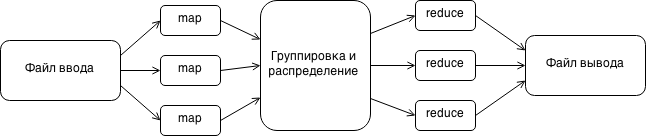
\includegraphics[scale=0.7]{mapreduce.png}
            \caption{Схематическое изображение обработки данных с помощью концепции map-reduce}
            \label{pic:mapreduce}
        \end{figure}

        На рисунке~\ref{pic:mapreduce} схематически изображена обработка данных с помощью map-reduce. Файл ввода разбивается на блоки, каждый из которых поступает на вход функции $map$. Функция map обрабатывает его и порождает список пар (ключ, значение). Множество полученных списков пар объединяется и, затем, группируется по ключу, получая для каждого ключа список всех ассоциированных с ним значений. Все ключи равномерно распределяются на блоки и передаются на вход стадии $reduce$. Стадия $reduce$ преобразовывает ключ и список значений в блок, являющийся частью файла вывода.

        Как видно из описания, концепция налагает ограничения на формат файлов ввода и вывода: данные должны быть коммуникативны, с некоторой точностью (обычно до строки).
    \clearpage

        \subsubsection{Проблемы, которые решаются с помощью map-reduce}
            Концепция map-reduce, появившись в 2004 году, довольно быстро обрела популярность, так как накопилось множество проблем для которых не существовало универсального решения. Вот основные из них~(в скобках указан подход к решению используемый в концепции map-reduce):

            \begin{itemize}
                \item вычисления превосходят возможности одной машины~(кластеры из сотен и тысяч машин),
                \item данные не помещаются в памяти, необходимо обращаться к диску~(последовательное чтение и запись намного эффективнее случайного доступа),
                \item большое количество узлов в кластере вызывает множество отказов~(все узлы унифицированы, что упрощает восстановление работы после отказа),
                \item данные хранятся на множестве машин~(данные обрабатываются на той же машине, на которой они хранятся),
                \item разработка низкоуровневных приложений для подобных систем --- дорого и сложно~(высокоуровневая модель программирования, универсальная и масшабируемая среда выполнения).
            \end{itemize} 

            В рамках курсового проекта была предложена реализация концепции, дающая решение только части поставленных выше проблем. Множество задач, решаемых в рамках реализованного фреймворка описано в главе~\ref{sec:tasks}.

        \subsubsection{Пример применения map-reduce}

            {\bfЗадача:} Есть граф пользователей некоторого ресурса, заданный в виде пар (пользователь, <<друг$_1$ друг$_2$ ...>>). Для каждой пары пользователей найти общих друзей.

            Разбор решения задачи будет проводится для следующих входных данных: 
            \lstset{} %TODO надо ли подписывать или и так сойдёт?
            \begin{lstlisting}[mathescape] 
    (A, B C D)
    (B, A C)
    (C, A B D)
    (D, A C)
            \end{lstlisting}

            Пусть функция map преобразовывает пару (пользователь, друзья) в множество пар.
            Для каждого друга формируется пара (ключ, значение) следующим образом: ключ~---~строка <<пользователь друг>>, если строка <<пользователь>>~$>$~строки <<друг>>, иначе строка <<друг пользователь>>, значение~---~<<друзья>>. Выполнения функции map в формате (входные даннные $\rightarrow$ результат):

            \lstset{}
            \begin{lstlisting}[mathescape] 
    (A, B C D) $\rightarrow$ [(A B, B C D), (A C, B C D), (A D, B C D)]
    (B, A C) $\rightarrow$ [(A B, A C), (B C, A C)]
    (C, A B D) $\rightarrow$ [(A C, A B D), (B C, A B D), (C D, A B D)]
    (D, A C) $\rightarrow$ [(A D, A C), (C D, A C)]
            \end{lstlisting}
                
            По выполнении функции map происходит подготовка данных для функции reduce, а именно множество полученных пар аггрегируется по ключу:

            \lstset{}
            \begin{lstlisting}[mathescape] 
    (A B, [B C D, A C])
    (A C, [B C D, A B D])
    (A D, [B C D, A C])
    (B C, [A B D, A C])
    (C D, [A B D, A C])
            \end{lstlisting}

            Функция reduce пересекает все элементы списка значений. Выполнения функции reduce в формате (входные даннные $\rightarrow$ результат):

            \lstset{}
            \begin{lstlisting}[mathescape] 
    (A B, [B C D, A C]) $\rightarrow$ (A B, C)
    (A C, [B C D, A B D]) $\rightarrow$ (A C, B D)
    (A D, [B C D, A C]) $\rightarrow$ (A D, C)
    (B C, [A B D, A C]) $\rightarrow$ (B C, A)
    (C D, [A B D, A C]) $\rightarrow$  (C D, A)
            \end{lstlisting}


        По выполнении функции reduce получили множество пар (ключ значение), где ключ~----~пара пользователей, значение~---~множество общих друзей:

            \lstset{}
            \begin{lstlisting}[mathescape] 
    (A B, C)
    (A C, B D)
    (A D, C)
    (B C, A)
    (C D, A)
            \end{lstlisting}

    \clearpage

    \subsection{Распределённая файловая система}
        {\it Распределённая файловая система~(РФС)}~---~файловая система, в которой данные хранятся на нескольких узлах. 

        В рамках реализации фреймворка map-reduce, РФС требуется для хранения одного файла в виде нескольких блоков, распределённых по нескольким узлам, а также для создания файла из блоков данных, расположенных на нескольких машинах.

        Распределённая файловая система является вспомогательным компонентом, поверх которого работает map-reduce. В рамках данной работы рассматривалась упрощенная модель файловой системы, которая обеспечивает все потребности map-reduce, но при этом не обладает важными возможностями файловых систем, такими как расширенные характеристики файлов и реплицируемость.

        В рамках работы была разработана РФС, которая позволяет хранить файлы, упорядоченные с помощью древовидной структуры каталогов. Файл представляет собой именованную последовательность блоков данных, которые распределены по нескольким узлам. Файл бьётся на блоки равного размера~(64 мб) с точностью до переносов строк.

        \begin{figure}[h!]
            \centering
            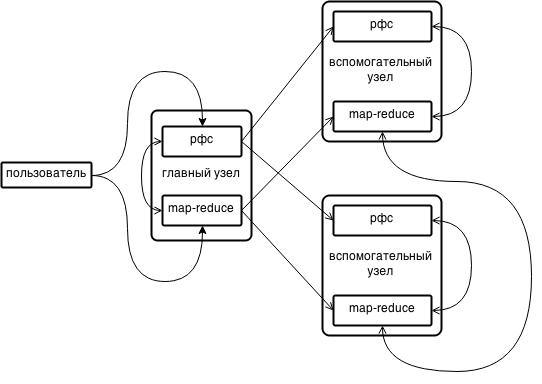
\includegraphics[scale=0.75]{framework_total.png}
            \caption{Взаимосвязь узлов при работе фреймфорка map-reduce}
            \label{pic:framework}
        \end{figure}
        
        На рисунке~\ref{pic:framework} показана общая архитектура фреймворка map-reduce. Рассмотрим часть, связанную с РФС.
        Пользователь работает с элементом РФС расположенном на главном узле, на котором хранится структура файловой системы и информация о блоках, составляющих каждый файл.
        Вспомогательные узлы хранят блоки и имеют интерфес, благодаря которому можно создавать, получать, удалять и переименовывать блоки.
    \clearpage
    \subsection{Распределённый map-reduce}
        Определение.

        map-reduce удобная концепция, но ... ??

        На рисунке~\ref{pic:framework} показана общая архитектура ...

        Описание этой архитектуры.

        \begin{figure}[h!]
            \centering
            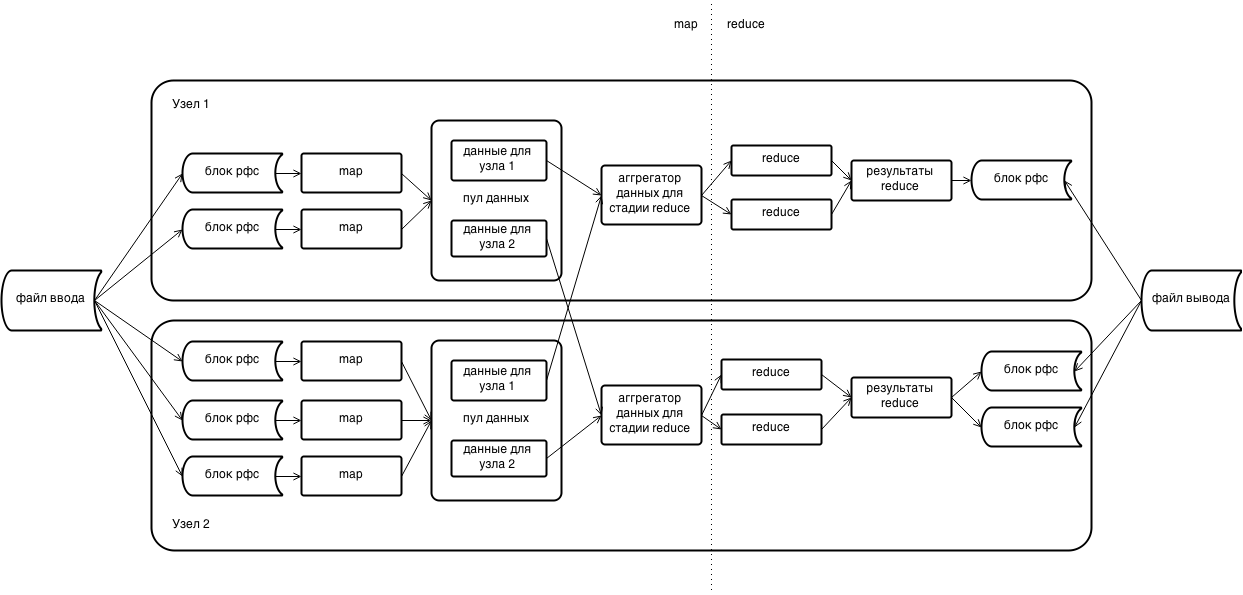
\includegraphics[scale=0.5,angle=90,origin=c]{map_reduce_framework.png}
            \caption{Схема выполнения приложения с помощью фреймфорка map-reduce}
            \label{pic:mr_framework}
        \end{figure}
        
        Подробное описание картинки.
        
    \clearpage

    \subsection{Решаемый класс задач}
    \label{sec:tasks}
        Необходимо обосновать существование и найти класс задач (здесь и далее под классом подразумевается некоторое множество задач), для которого актуальна приведённая выше схема распределённого map-reduce.

        Пусть каждый узел располагает $memory$ доступной оперативной памяти (здесь и далее единицей измерения памяти будет байт) и $storageSize$ свободного места на диске. Всего узлов $numNodes$. Данный map-reduce проектировался для решения задач с {\it большими данными}, поэтому в дальнейшем будем считать, что входные данные $>>memory$. 

        \subsubsection{Oграничения на стадии map и reduce}
            На вход стадия map принимает данные с диска, а результат этой стадии равномерно (с точностью до пары (ключ, значение)) распределяется по оперативной памяти узлов. То есть входные данные $<storageSize*numNodes$, а результат $<< memory*numNodes$. Так как $storageSize >> memory$, получаем, что, в общем случае, стадия map должна сильно сокращать объём данных.

            На вход стадия reduce принимает данные из оперативной памяти, которые $<< memory*numNodes$, результат этой стадии аккумулируется в оперативной памяти, то есть должен быть $<<memory$ для каждого узла, а затем записывается на диск. Получаем, что стадия reduce должна, как минимум, не увеличивать объём данных, поступивших на вход.

            Рассмотрев полученные выше ограничения для стадий map и reduce, а также учитывая достаточно большие входные данные, можно увидеть, что распределённый map-reduce оптимально подходит для решения задач класса {\it информационный поиск} ({\it information retrieval}), что является одним из этапов решения задач {\it анализа данных} ({\it data mining}).

            {\it Информационный поиск} --- процесс поиска и получения информации как из структурированных, так и из неструктурированных данных. Обычно применяется в {\it анализе данных} для первичной обработки и сокращения объёма исходных данных. 

        \clearpage

        \subsubsection{Пример задачи класса информационный поиск}

            Исходные данные хранятся в виде текстового файла в $n$ строк, в котором каждая строка соответствует строке в реляционной таблице $table$ с $m$ столбцов ($f_1...f_m, m>2$), каждое значение записано через пробел. Необходимо получить результат выполнения SQL запроса:
            \lstset{language=SQL}
            \begin{lstlisting}[mathescape] 
    SELECT $f_1, ..., f_m$
    FROM $table$
    WHERE $f_1 > const$
    GROUP BY $f_1$
            \end{lstlisting}

        \subsubsection{Решение задачи с помощью фреймворка map-reduce}
            
            Функция map определяется следующим образом: для каждой строки проверяется условие {\bf WHERE} и все строки, удолетворяющие условию, составляют результат в виде пар: $(f_1, f_2, ..., f_m)$. Количество строк, удолетворяющих условию {\bf WHERE}, обозначим как $n'$. Функция reduce возвращает то, что получила на вход.

            Стадия map получает $O(nm)$ данных и, по выполнении, выдаёт $O(n'm)$ данных, которые преобразуются и без изменений проходят стадию reduce. Сложность стадии map --- $O(nm)$, преобразования между стадиями --- за $O(n'm+n'ms_{net})$ ($s_{net}$ --- стоимость передачи данных между узлами), стадии reduce --- $O(n')$. 

        \subsubsection{Решение задачи на одной машине}
            Решение задачи одной машине без применения фреймворка состоит из двух стадий: 
            \begin{itemize}
                \item получить из входного файла все строчки, удолетворяющие {\bf WHERE} --- сложность $O(nm)$ (по памяти $O(n'm)$)
                \item сгруппировать полученный результат по ключу $f_1$ --- сложность $O(n'ln(n'))$, если применить для аггрегации быструю сортировку (по памяти $O(n'm)$), сложность $O(n')$, если применить для аггрегации сортировку подсчётом (по памяти $2O(n'm)$).
            \end{itemize}

            В случае когда $n'$ и $m$ определены таким образом, что получишиеся данные больше $memory$, возникают проблемы: необходимо сохранять на диск промежуточные результаты, полученные после первой стадии, и сортировать полученный результат на диске, что достаточно медленно. В наиболее быстром варианте (результат первой стадии по частям сортируется и сохраняется файлах, а затем эти файлы сливаются) получается сложность первой стадии --- $O(nm+n'ln(n')+n's_{hdd})$, второй стадии $O(n'ms_{hdd})$ ($s_{hdd}$ --- стоимость обращения к диску).

        \subsubsection{Выводы}
            Cуммарная сложность решения с помощью map-reduce --- $O(nm+n'm+n'ms_{net}+n')$, с помощью описанного выше способа решения на одной машине --- $O(nm+n'ln(n')+n's_{hdd}+n'ms_{hdd})$. Можно увидеть, что по сложности данные алгоритмы принципиально не отличаются (в обоих случаях сложность $O(nm)$) за исключением двух важных моментов (их влияние будет оценено в главе \ref{sec:tests}):
            \begin{itemize}
                \item обычно $s_{net}>>s_{hdd}$,
                \item время выполнения на одной машине существенно увеличивается за счёт последовательного выполнения всех действий, которые происходят параллельно в случае map-reduce.
            \end{itemize}

            Также необходимо отметить, что решение задачи на одной машине осложняется реализацией механизмов, альтернатива которых уже реализована в фреймворке. 

            В итоге можно сказать, что предложенная схема реализации концепции map-reduce позволяет решать задачи класса информационный поиск. Эффективность решения таких задач оценена в главе \ref{sec:tests}.
        
    \clearpage
\clearpage

\section{Объекты и методы}      
        \noindent Характеристики программного обеспечения:
        \begin{itemize}
            \item Операционная система --- Ubuntu 14.04.1 LTS 64-bit.
            \item IDE --- Syblime Text 2.
            \item Язык программирования --- Python 2.7.3.
        \end{itemize}
        
        \noindent Характеристики оборудования:
        \begin{itemize}
            \item Процессор --- Intel Core i7-3770k 3.5Ghz$\times$8.
            \item Оперативная память --- 16Gb DDR3.
            \item Видеокарта --- ATI Radeon 7860.
        \end{itemize}
\clearpage

\section{Реализация}
    \subsection{Используемые технологии}
        При реализации ... были использованы готовые технологиии: ...

        \subsubsection{Коммуникация по сети}
            что такое

            зачем нужно

            почему zmq

        \subsubsection{Сериализация}
            что такое

            зачем нужно

            примеры, тесты

            почему выбрали marshal

            Cериализация в человекочитаемый формат % TODO человекочитаемый

            что такое и чем отличается от сериализации

            json и xml определение и зачем нужно

    \clearpage

    \subsection{Работа с большими данными}

        какие есть проблемы - описать все нижни пунксты

        \subsubsection{python generator}
            Рассказ про python generator

            и применение

        \subsubsection{split}
            обзор функции split

        \subsubsection{dfs}
            проблемы в dfs ?? доопределиться по ходу написания

            как эти проблемы решаются в фс
        \subsubsection{map-reduce}
            проблемы в map-reduce ??

            распределение ключей

            как эти проблемы решаются в map-reduce
    \clearpage 

    \subsection{Взаимодействие между узлами}

        Описание реализации взаимодействия между различными узлами сети.

        класс nodesmanager и примеры его использования

    \clearpage

    \subsection{Интерфейс}

        есть dfs, есть mr

        \subsubsection{dfs}
            перевести

            Distributed file system is required to map-reduce framework.

            On each node, you should run *dfsnode.py* with two arguments - port and storagepath. Like this:


                python dfsnode.py -p 5556 -s /home/username/storage


            Then you should fill *config.json* with information about nodes. Now you can use *dfs.py*. Samples of use dfs.py:


                python dfs.py -ls /user/
                python dfs.py -mkdir /user/username/userdatafolder
                python dfs.py -put ./test.in /user/username/userdatafolder/testfile
                python dfs.py -get /user/username/userdatafolder/testfile
                python dfs.py -rm /user/username
        \subsubsection{mr}
            написать аналогично dfs
    \clearpage  


\clearpage

\section{Тестирование}
\label{sec:tests}
    бла бла
        
\clearpage

\section{Заключение}

    Описать успех или не успех тестирования. 

    Описать проблемы. 

    Описать удачи.
    
\clearpage


\begin{thebibliography}{0}
\addcontentsline{toc}{section}{Список литературы}
    \bibitem{smth}
    гугловая статья про mr от 2006

    лекции шад http://www.slideshare.net/yandex/mapreduce-12321523

    http://www.quora.com/What-is-the-most-efficient-way-to-serialize-in-Python

    http://www.codeinstinct.pro/2012/08/hadoop-design.html

    https://highlyscalable.wordpress.com/2012/02/01/mapreduce-patterns/

    \bibitem{SMILES}
         SMILES~---~A Simplified Chemical Language~//~Daylight Chemical Information Systems, Inc: URL: http://www.daylight.com/dayhtml/doc/theory/theory.SMILES.html
    \bibitem{PDBformat}
        Atomic Coordinate Entry Format Description~//~Penn State University: URL: http://www.wwpdb.org/documentation/format33/v3.3.html
        
    \bibitem{PSU}
        Periodic Table Datan Files~//~Protein Data Bank: URL: http://php.scripts.psu.edu/djh300/cmpsc221/p3s11-pt-data.htm
    \bibitem{threejs}
        Three.js~---~javascript 3D library~//~Three.js: URL: http://mrdoob.github.io/three.js/
        
    \bibitem{wikiribbon}
       File: Tubby-1c8z-pymol.png~//~Wikipedia: URL: http://en.wikipedia.org/wiki/File:Tubby-1c8z-pymol.png
             
    \bibitem{GLMol}
       GLmol - Molecular Viewer on WebGL/Javascript~//~GLmol: URL: http://webglmol.sourceforge.jp/index-en.html
        
\end{thebibliography}

\end{document}




